\documentclass{../source/Experiment}

\major{信息工程}
\name{姚桂涛}
\title{卷积神经网络}
\stuid{3190105597}
\college{信息与电子工程学院}
\date{\today}
\lab{教11-400}
\course{人工智能实验}
\instructor{胡浩基、魏准}
\grades{}
\expname{卷积神经网络}
\exptype{设计验证}
\partner{}
\begin{document}
    \makecover
    \section{实验题目}
        \subsection{实验7-1}
        通过给定的 Pool 、 Conv 和 LoadMnistData 函数
        通过 momentum 规则,对 上述卷积神经网络进行训练
        
        采用 训练数据:测试数据 8:2 的 比例(训练数据
        2000 ),进行 训练和测试,并 输出 训练后预测结
        果的准确度。  

    \section{实验结果}
        \subsection{实验6-1}
            均方误差:loss= 0.0012654705817646574
            准确率:0.932
            可视化结果:
            \begin{figure}[H]
                \centering
                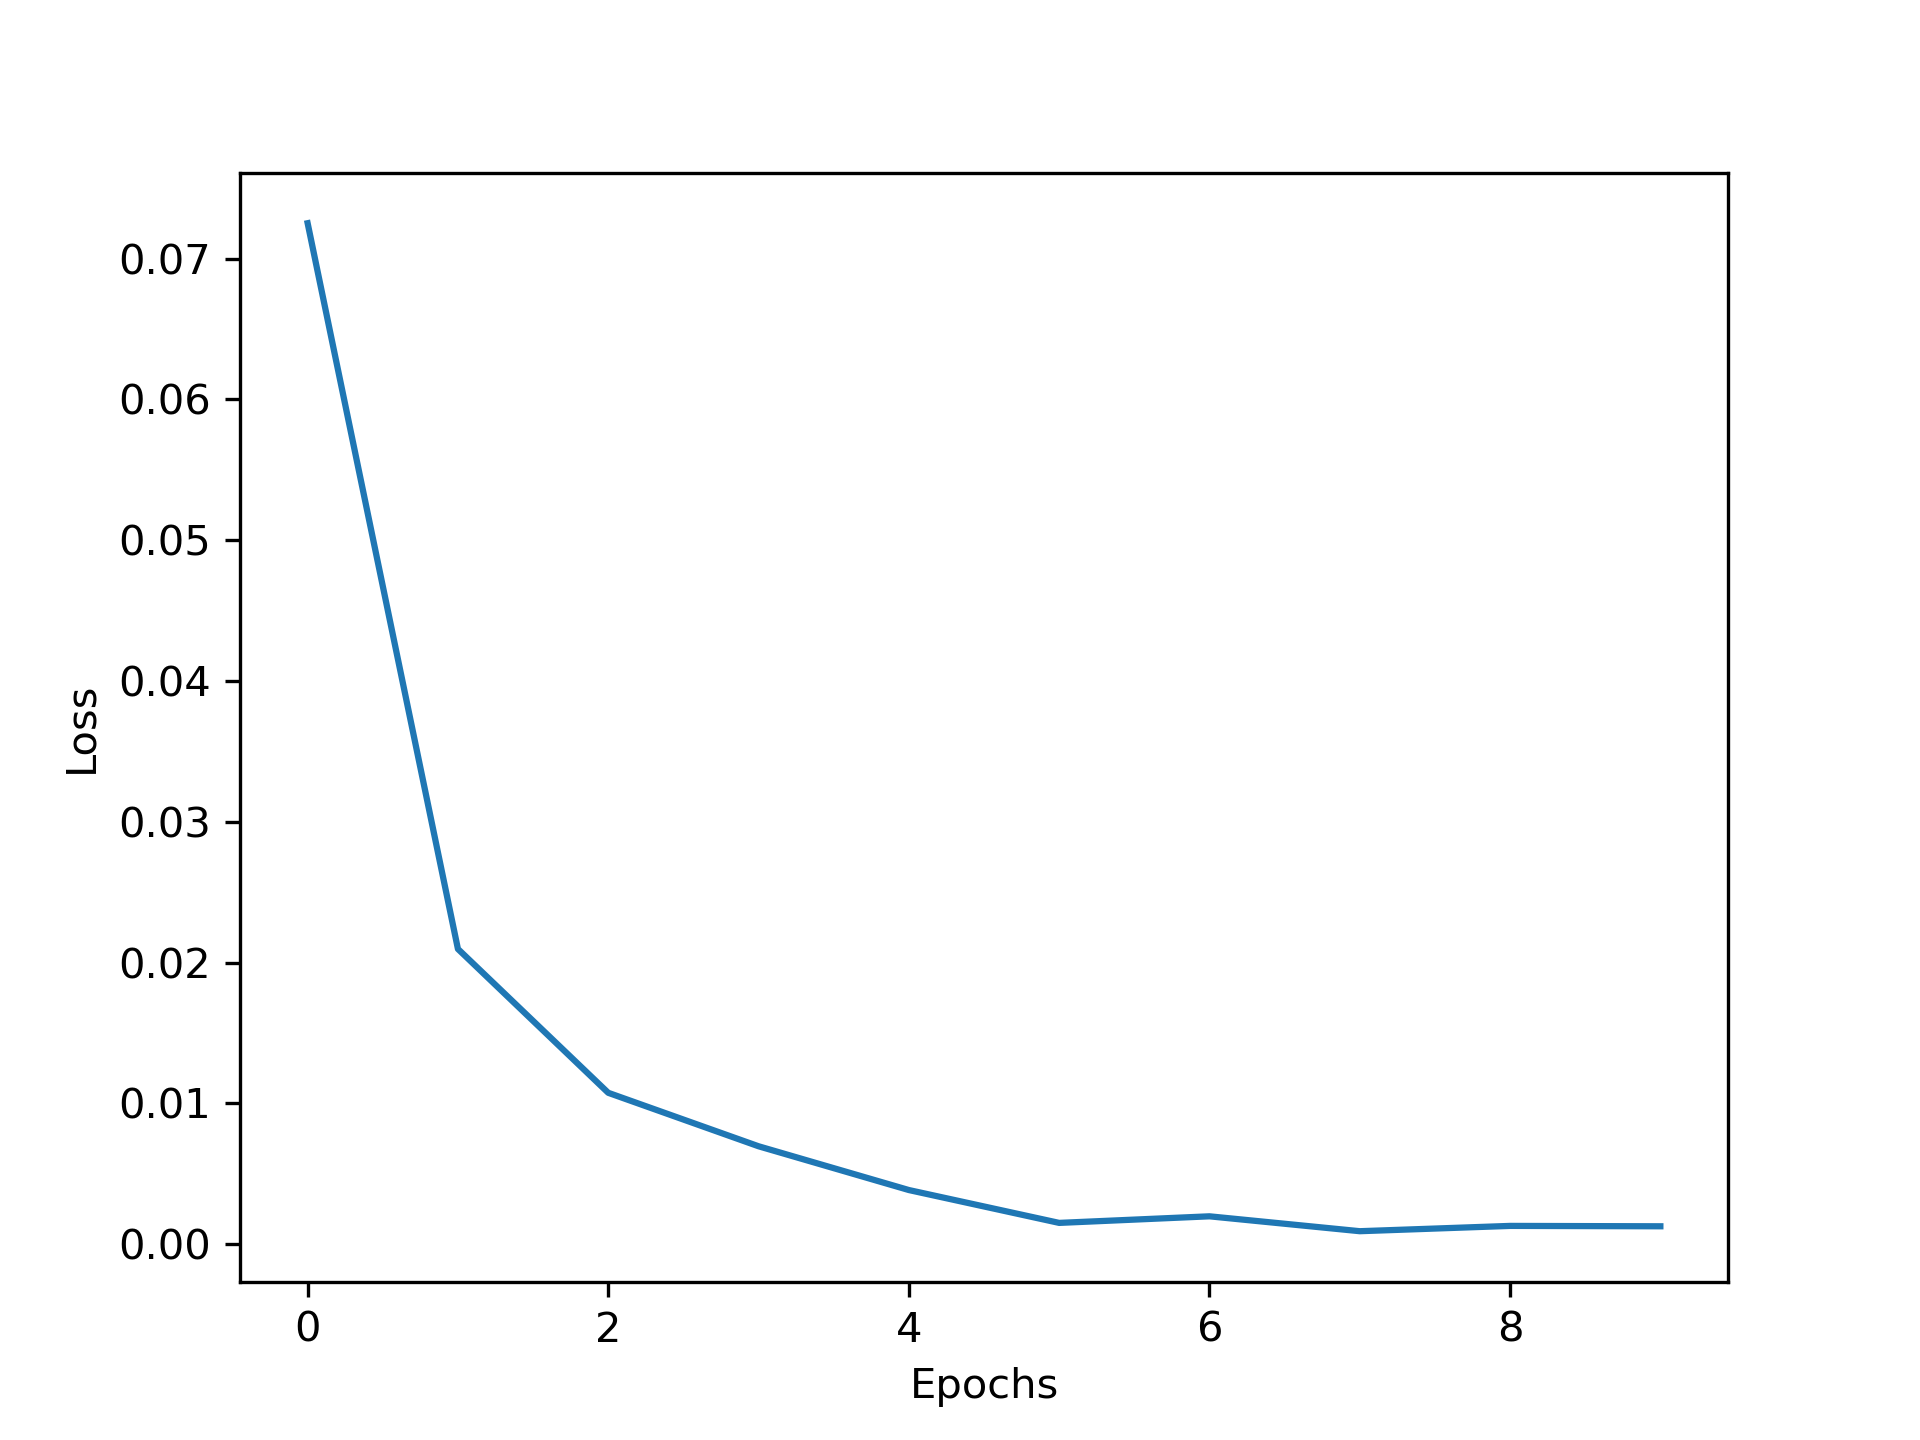
\includegraphics[width = 0.6\textwidth]{Part7/lab10_by_zyl/lab7_1.png}
                \caption{可视化}
            \end{figure}

\end{document}


